\documentclass[runningheads]{llncs}

\usepackage[T1]{fontenc}
\usepackage{graphicx}
\usepackage{url}

\begin{document}

\title{Network-Level Insights into Google-Free Android Operating Systems}

\author{Bruno Mirčevski\inst{1}\orcidID{0009-0007-1008-6708} \and
Second Author\inst{1}\orcidID{1111-2222-3333-4444}}

\authorrunning{B. Mirčevski et al.}

\institute{Faculty of Computer Science, Bialystok University of Technology, Wiejska 45a, 15-351, Bialystok, Poland}

\maketitle

\begin{abstract}
This paper presents a comparative analysis of privacy in Android operating systems through network traffic inspection. Using a controlled man-in-the-middle setup and traffic decryption techniques, six Android distributions were evaluated: stock Google Android, GrapheneOS, iodéOS and LineageOS (stock, Gapps, microG). The study examined outbound connections, transmitted identifiers, and network traffic patterns to assess the impact of integrated Google services on user privacy. Results indicate that stock Android maintains the most communication with Google servers, transmitting identifiers and metadata even when idle. In contrast, privacy-focused systems minimize unsolicited traffic and offer stronger user control. The findings demonstrate that alternative Android distributions can substantially improve privacy without sacrificing core functionality, highlighting the potential of open-source ecosystems as viable, privacy-respecting alternatives to Google-dependent mobile environments.

\keywords{Android  \and Privacy \and Network traffic.}
\end{abstract}

% ---- Content ----

\section{Introduction}
Android is the dominant mobile operating system and acts as a primary gateway to digital world for billions of users. It's crucial for core OS to be a reliable, stable and trustworthy platform, that allows users to run apps and services of their choice. While mobile app privacy has been widely studied \cite{appDataCollection1,appDataCollection2,appDataCollection3,appDataCollection4,firmwaredroid2023}, less attention is typically paid to the operating system layer and to privileged service frameworks that silently enable additional functionality. Standard unprivileged apps are constrained by Android's permission model, although some attempt to circumvent it in creative ways \cite{appDataCollection5Circumvention,appDataCollection6Circumvention}. In contrast, privileged system apps operate with higher access to the device and OS, which makes them harder to understand and control. Most user-facing privacy controls focus on applications and permissions, yet a substantial amount of data exchange can occur below the app layer, through OS services, vendor components, and Google service frameworks. This work therefore compares the network behavior of multiple Android distributions and their preinstalled/privileged system components under controlled, reproducible conditions.

\subsection{Android dependency on privacy-threatening services}
While Android’s core is the Android Open Source Project (AOSP), most consumer devices ship with additional proprietary components layered on top. They are often implemented as privileged system apps and service frameworks to provide baseline functionality such as push notifications, location assistance, app distribution/updates, device integrity checks and many more. Users and app developers commonly assume their presence and availability by default. 

These components exists for a practical reason. Centralized services can significantly improve usability and efficiency, for example by reducing battery drain compared to per‑app background connections, and by providing faster, more accurate location through fused network and sensor-based methods. However, this design also tightly couples many functions into a single service stack, so enabling useful capabilities may implicitly enable others that a user would not choose, such as advertising identifiers, telemetry, and behavioral tracking. In practice, the result is a large proprietary bundle that is difficult to audit and decompose into only the features a user actually wants.

On Android, these baseline capabilities are most commonly delivered through Google’s service stack. Because Google’s business model is strongly advertising-driven, many users may be unwilling to entrust this provider with broad access to device and their data. In principle, users should be able to choose which services they rely on and have confidence that these choices are enforced by the platform’s permission and isolation mechanisms. This demand for transparency and controllability motivates alternative approaches such as microG and GrapheneOS’ sandboxed Google Play. These solutions aim to preserve device functionality and app compatibility while reducing privilege and improving user control over Google-related components.

\subsection{Privacy-focused Android operating systems}
Privacy-focused Android operating systems (also referred to as \emph{custom ROMs}) are distributions derived from AOSP that aim to reduce data exposure at the OS level by limiting preinstalled privileged components, tightening default settings, and providing more transparent controls over permissions and network access. In contrast to many factory builds that bundle large proprietary service stacks, privacy-oriented systems typically try to (i) minimize default background communication, (ii) reduce the use of persistent identifiers, and (iii) give the user stronger enforcement mechanisms to disable or constrain components that are not strictly required for everyday use.

In this work we focus on three representative approaches. GrapheneOS prioritizes a hardened security model and strong isolation. Google components are not included by default, but can be installed in a dedicated sandboxed mode as ordinary apps, without the special privileges that Google Mobile Services (GMS) typically hold on factory systems. This design targets improved containment and user control while preserving high compatibility when the user decides to install Google services. 

LineageOS provides a lightweight, broadly supported AOSP-based system with minimal preinstalled software and extensive device compatibility. It can be deployed in multiple configurations: without Google services, with official proprietary Google Play Services and Play Store, or with microG as an open-source reimplementation of key Google APIs. These configurations represent different trade-offs between privacy, compatibility, and reliance on proprietary services. 

Finally, iod\'eOS is a privacy-oriented distribution based on LineageOS that combines a de-Googled baseline with additional privacy features and preconfigured app ecosystem choices, shipping with microG. For completeness, CalyxOS follows a similar privacy-oriented direction (AOSP-based, microG-enabled, and designed for practical daily use). It was considered for the study, but was excluded because it was not receiving updates during the measurement period.

\subsection{Challenges of network traffic analysis on Android}
Network traffic analysis on Android is difficult by design and that is largely a security benefit. Modern protocols increasingly hide data behind encryption (TLS 1.3, QUIC/HTTP3, encrypted DNS). Even when traffic is captured, compression and binary encodings can make payloads hard to interpret without schemas or additional context. As a result, MITM-based decryption is inherently incomplete. Certificate pinning and anti-tamper mechanisms can block interception or break app functionality. Circumvention of these security mechanisms do not reliably yield a full plaintext view. While prior work demonstrates these challenges in a reproducible emulator-based setup \cite{parrot2025}, this work uses a physical device to capture behavior under more realistic firmware, hardware, and service conditions. We accept that some flows will remain opaque, not all network communication will be revealed or understood. Our focus in on differences between studied Android systems and on general patterns.
\section{Related work}
Prior work has shown that privacy risks on Android extend beyond user-installed applications and can arise from the operating system layer and preinstalled components. Measurement studies of vendor-modified Android variants report background communication to OS vendors and third parties even under minimal configuration. Transmitted data includes persistent identifiers, app and device metadata, which creates possibility of re-linking resettable identifiers when they co-occur with long-lived identifiers \cite{android-os-snooping2021}. Other measurements report that Google Play Services and the Play Store store cookies, tokens, and device identifiers even in the absence of explicit user activity \cite{cookies-identifiers2025}. Broader ecosystem-level investigations further highlight how data collection can be driven not only by first-party apps and platforms, but also by advertising and analytics infrastructure (which is sometimes preinstalled), enabling linkage between nominally pseudonymous identifiers and user accounts \cite{google-data-collection2018}.

[Alternative OS are not well studied...]
\section{Experiment design}

\begin{figure}
	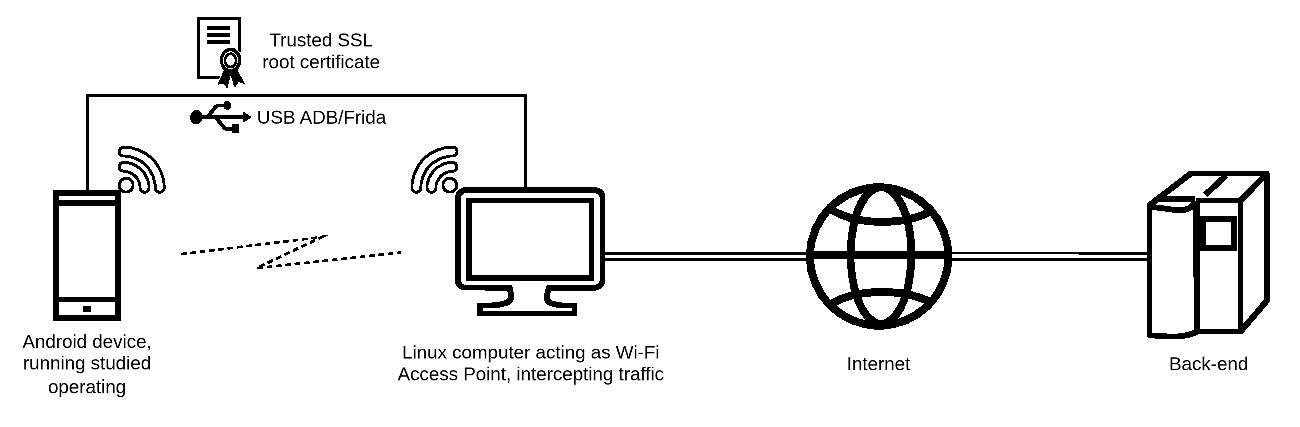
\includegraphics[width=\textwidth]{images/devices.eps}
	\caption{Measurement setup. Android device running studied operating systems is configured to access Internet using Wi-Fi. Access point is hosted on a Linux computer, running traffic interception and capturing software. Custom system certificate is installed on the phone using root access. USB connection is used for ADB/Frida communication.} \label{fig1}
\end{figure}

\subsection{Measurement Scenarios}
To enable consistent, comparable measurements across Android distributions, four setup scenarios were defined. Each scenario specifies (i) Google account state, (ii) consent/permission posture, and (iii) what Google components are present. Not all scenarios apply to every operating system due to their characteristics.

\paragraph{Scenario A: Default Setup with Google Account.}
The device is configured to reflect a typical user path. Google account sign-in is performed during setup (or immediately after) and default recommendations are accepted (including permissions).

\paragraph{Scenario A2: Minimal Setup with Google Account.}
This scenario applies exclusively to the official factory system. It extends \textit{Scenario A} by systematically minimizing privacy exposure while retaining Google account functionality. During and after initial setup, all optional consents and permissions are declined. System and account settings are adjusted to maximize user privacy. This scenario is not applicable to alternative distributions, as these systems are configured for privacy by default and do not implement or prompt users for privacy-threatening features characteristic of the factory system.

\paragraph{Scenario B: Minimal Setup without Google Account.}
The device is configured with maximum privacy in mind, avoiding Google account sign-in entirely. During initial setup, only strictly required prompts are accepted and optional data-sharing is declined. System settings are  adjusted to maximize user privacy. Google components or their functional replacements remain present and enabled to preserve baseline device functionality and app compatibility, but operate without account.

\paragraph{Scenario C: Extremely Minimal Setup without Google Components.}
This scenario applies only to distributions that do not bundle or enable Google components by default. The device is configured to operate without any Google Mobile Services, sandboxed Google Play, or microG. On GrapheneOS, this configuration is achieved by declining installation of Google components during initial setup; on LineageOS and iod\'eOS, microG is present but explicitly disabled. This scenario is not applicable to the official factory system, which bundles and enables Google components by default.

[Scenario adaptation to microg/graphene...]
\section{Results}

\subsection{Data usage across operating systems and scenarios}

Total network data usage across all operating systems and applicable scenarios for performed tasks, is presented on charts in Figures~\ref{fig-setup-chart}--\ref{fig-apps-chart}. To keep the results comparable and avoid dominance by bulk transfers, we excluded traffic to domains used for app and system update payload delivery (large binary downloads), though this exclusion was not perfect and some residual update-related traffic remains in the dataset. Generally, we expect lower network traffic in configurations with fewer Google services present.

\begin{figure}
	\includegraphics[width=\textwidth]{images/setup-data-usage.eps}
	\caption{Task 0: Initial setup data usage} \label{fig-setup-chart}
\end{figure}

Figure \ref{fig-setup-chart} illustrates network activity during initial device setup. As expected, stock Android exhibits the highest data usage. The modest reductions between privacy-adjusted scenarios indicate that configuration choices provide little control over automatic updates and background synchronization. Across all distributions, variations align with service architecture: configurations incorporating more Google services generate proportionally higher traffic, while de-Googled baselines demonstrate substantially reduced exchange. LineageOS with official Google Play Services generates substantially less traffic than stock Android due to its more minimal base system, yet remains considerably higher than configurations without proprietary Google services, with the microG variant and Google-free installation achieving notable further reductions. On GrapheneOS, Scenario B demonstrates that even when sandboxed Google Play Services are installed and granted network and background permissions, they remain largely inactive when not deliberately invoked, contrasting sharply with the persistent background activity characteristic of integrated GMS deployments.

\begin{figure}
	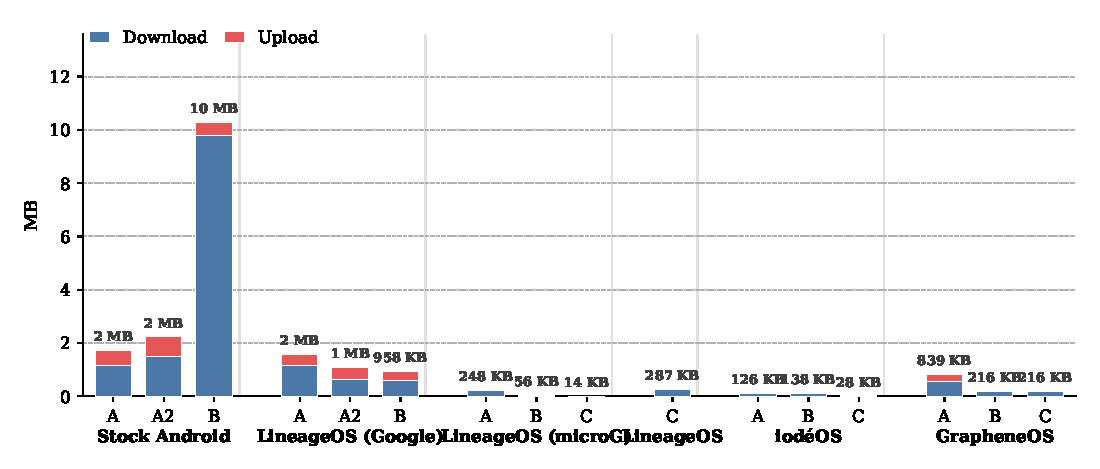
\includegraphics[width=\textwidth]{images/idle-data-usage.eps}
	\caption{Task 1: Idle data usage} \label{fig-idle-chart}
\end{figure}

Network activity observed during system idle following a reboot is presented in Figure \ref{fig-idle-chart}. Stock Android again shows the highest data usage, though Scenario B exhibits unexpectedly elevated traffic compared to both Scenario A2 and Scenario A. This anomaly stems from substantial background communication with www.gstatic.com, likely triggered by automatic updates or application background activity during the measurement time.

LineageOS in Scenario C similarly deviate from anticipated patterns, generating more idle traffic than its microG variant. LineageOS made connections to agnss.goog (Google Assisted GNSS) and www.gstatic.com. The agnss.goog endpoint was also observed in LineageOS (microG) during other measurement tasks, indicating that the entire LineageOS family retains this Google-dependent location mechanism. Other alternative distributions either replace this component with independent implementations or allow users to disable it entirely. GrapheneOS exhibits virtually identical idle traffic in Scenarios B and C, confirming that sandboxed Google Play Services remain dormant when not actively invoked.

\begin{figure}
	\includegraphics[width=\textwidth]{images/apps-data-usage.eps}
	\caption{Task 2: Basic apps interactions data usage} \label{fig-apps-chart}
\end{figure}

Figure~\ref{fig-apps-chart} shows network activity during basic app interactions that should not require Internet connectivity. Stock Android dominates with substantial data usage mostly by uncontrolled updates. All alternative distributions demonstrate dramatically lower traffic, with de-Googled configurations remaining effectively silent. Notably, whenever official Google Play Services were present and a Google account logged in at least a single request to Google infrastructure occurred.

\subsection{Domain distribution and Google dependencies}

\begin{figure}
	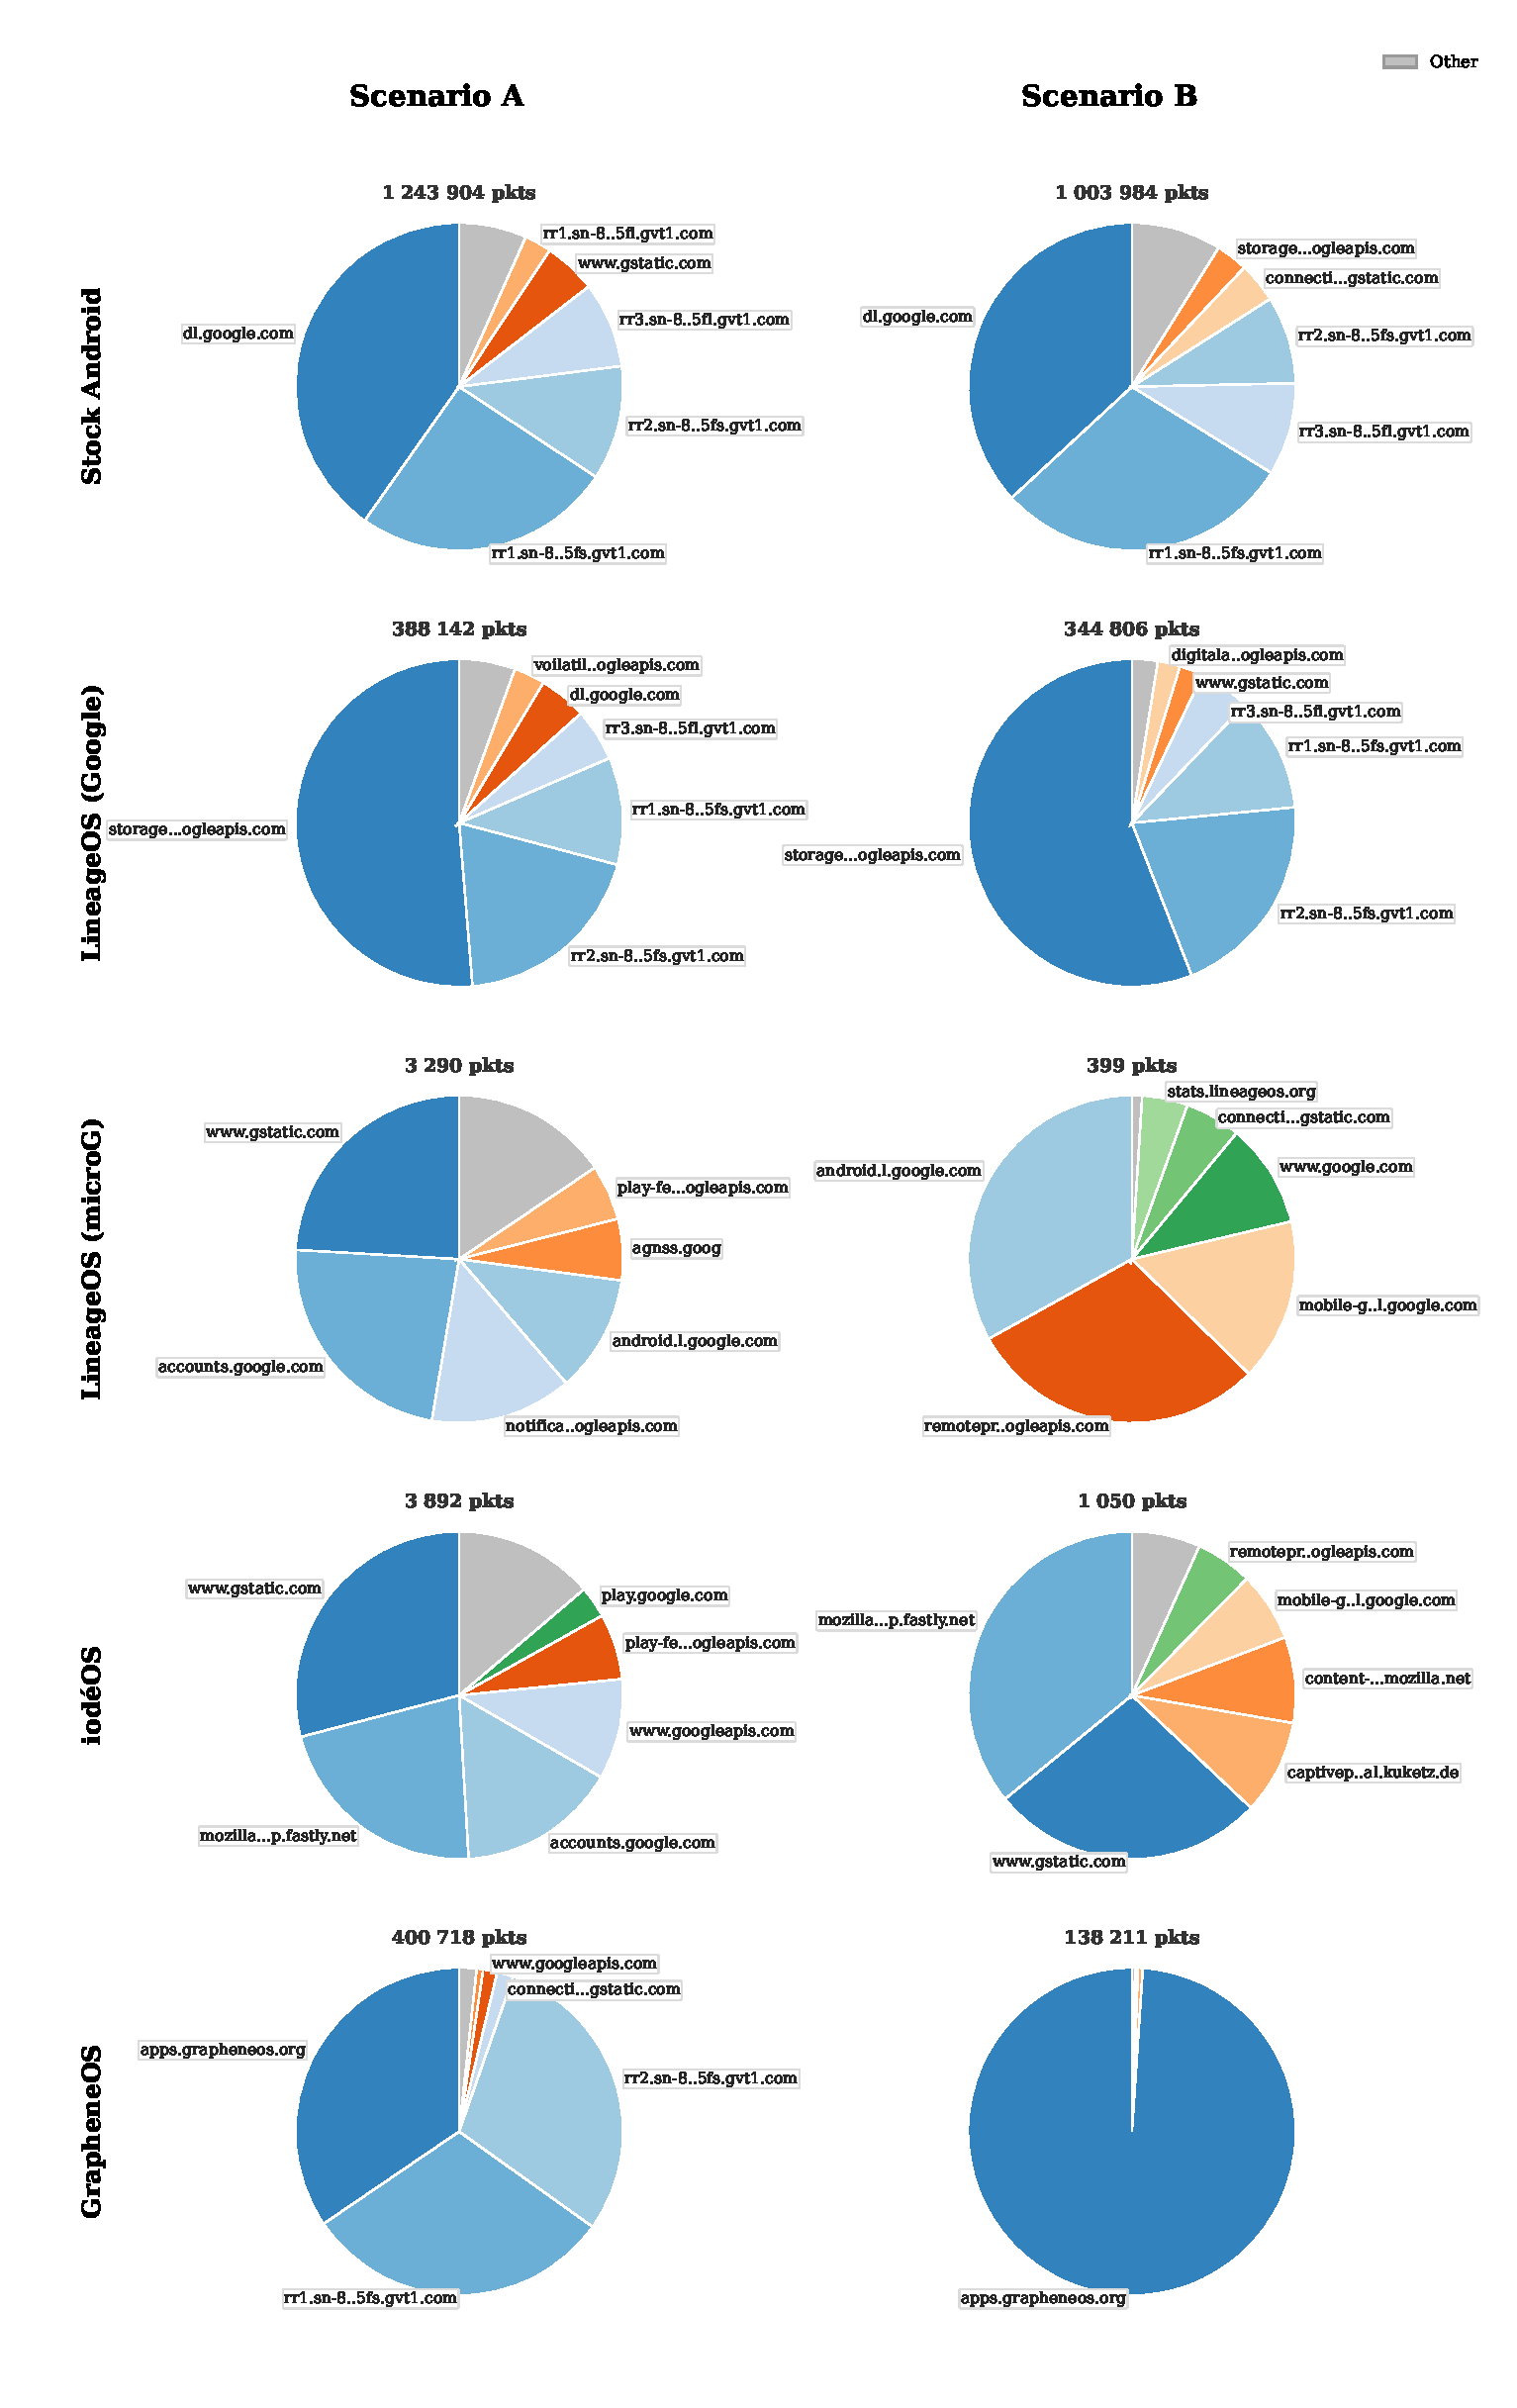
\includegraphics[width=\textwidth]{images/domains.eps}
	\caption{Domain-level distribution of network packets for scenarios A (with Google account) and B (without Google account, but Google Services present), aggregated over all tasks. Each pie shows the top domains by packet count for a given operating system and scenario.} \label{fig-domains-chart}
\end{figure}


[Lineageos uses SUPL from google, explain remoteprovisioning.googleapis.com, graphene makes no google connections by default, connectivity check is google on lineage]

[Table comparing google domains with replacements from other systems]
\section{Conclusion}

[Based on requests google can determined if device is running stock os, or microg or graphene]
[Adjusting Privacy settings matters, it makes difference, but for higher privacy levels alternative OS is required]
[All alternative OS do not force EULA]

% ---- Bibliography ----
\bibliographystyle{splncs04}
\bibliography{refs}

\end{document}
